\documentclass[reprint,amsmath,amssymb,aps]{revtex4-2}

\usepackage{graphicx} % Include figure files
\usepackage{dcolumn} % Align table columns on decimal point
\usepackage{bm} % bold math
\usepackage{hyperref} % add hypertext capabilities
\usepackage[spanish,mexico]{babel}
\usepackage{float} %usar [H]
\usepackage{diagbox}
% \graphicspath{{imagenes/}} %Carpetas donde estaran las imagenes

\begin{document}

\preprint{APS/123-QED}

\title{Template-based Routing Generator}
\author{José de Jesús de la Rosa de la Rosa}
\email{a228835@alumnos.uaslp.mx}
\affiliation{Facultad de Ciencias, Universidad Autónoma de San Luis Potosí.}
\date{22 de junio de 2022}

\begin{abstract}

\end{abstract}

%\keywords{HOLA,JH,OK}

\maketitle 

\section{Introducción}

Durante años se han propuesto en la literatura técnicas de enrutamiento para la automatización del diseño de circuitos integrados (IC) digitales y analógicos. En ellas, ya se ha cubierto un amplio conjunto de restricciones geométricas para la la mejora de calidad del enrutamiento, pero también se han incluido progresivamente criterios relacionados con el rendimiento. Sin embargo, a medida que el diseño de circuitos mas complejos y de características particulares, como en los circuitos analógicos y de radiofrecuencia, avanzan hacia nuevos nodos tecnológicos, el creciente número de reglas y restricciones de diseño, la resistencia de cables, la congestión y el crecimiento de circuitos parasíticos entre cables, impulsan constantemente las técnicas de enrutamiento automático existentes y mantienen la presión sobre su mejora.

En la literatura se han propuesto técnicas de enrutamiento para la automatización del diseño de circuitos integrados analógicos y de radiofrecuencia (A/RF)~\cite{unutulmaz, martins}. En ellas, ya se ha cubierto un amplio conjunto de restricciones geométricas como sustitutos de la calidad del enrutamiento, pero también se han incluido progresivamente criterios relacionados con el rendimiento. Sin embargo, a medida que el diseño de circuitos A/RF avanza hacia nodos tecnológicos de integración avanzada, el creciente número de reglas ó restricciones de diseño, la resistencia de los cables, la congestión y el crecimiento parasitario entre cables desafían constantemente las técnicas de enrutamiento automático existentes y mantienen la presión sobre su mejora. Afortunadamente, los recientes avances en las capacidades de las estaciones de trabajo modernas permitieron el crecimiento de sofisticados procesos de enrutamiento, incluidos algunos asistidos por los últimos métodos de aprendizaje automático y profundo, que ofrecen soluciones sin precedentes para la automatización de esta tarea. Sin embargo, la correlación entre las estructuras parasíticas inducidas por el enrutamiento y el comportamiento funcional del circuito dista mucho de ser sencilla, también se han propuesto técnicas de síntesis computacionalmente intensivas con inclusión de parásitos y conscientes del diseño, en las que las técnicas de enrutamiento automático desempeñan un papel decisivo.\\

\section{Path-finding algorithm}

Una de las principales técnicas es el uso de generadores de enrutamiento basados en plantillas (TbRG, \textit{Template-based routing generators}). La plantilla actúa como una representación del diseño gráfico de la tecnología, generada por el conjunto y características de los dispositivos. Son especialmente útiles cuando se debe migrar un diseño validado previamente diseñado, es decir, un diseño heredado, a otros nodos de tecnología cercanos o se necesitan cambios en el diseño. Esta plantilla puede ser implementada como un grafo de pesos unitarios, conexo y no dirigido, donde se seleccionan un vértice origin y destino, y a través de diferentes algoritmos, encontrar el camino mas corto.

El algoritmo de Dijkstra, también llamado algoritmo de caminos mínimos, es un algoritmo para la determinación del camino más corto, dado un vértice origen, hacia el resto de los vértices en un grafo que tiene pesos en cada arista. La idea general en este algoritmo consiste en ir explorando todos los caminos más cortos que parten del vértice origen y que llevan a todos los demás vértices, cuando se obtiene el camino más corto desde el vértice origen hasta el resto de los vértices que componen el grafo, el algoritmo se detiene. Se trata de una especialización de la búsqueda de costo uniforme y, como tal, no funciona en grafos con aristas de coste negativo (al elegir siempre el nodo con distancia menor, pueden quedar excluidos de la búsqueda nodos que en próximas iteraciones bajarían el costo general del camino al pasar por una arista con costo negativo).

Existe una variante del algoritmo de Dijkstra, llamado algoritmo A*, el cual tiene como objetivo únicamente el camino más corto desde una fuente específica hasta un objetivo específico, y no el árbol de caminos más corto desde una fuente específica hasta todos los objetivos posibles. Para esto es es necesario el uso de una función heucarística. Para el algoritmo de Dijkstra, dado que se genera todo el árbol de la ruta más corta, cada nodo es un objetivo y no puede haber una heurística dirigida a un objetivo específico, obteniendo peor rendimiento que el algoritmo A* cuando la búsqueda del camino mas corto es solo entre dos nodos.

 \begin{figure}[H]
 	\centering
 	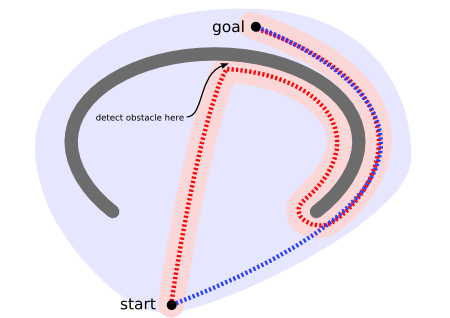
\includegraphics[width=0.48\textwidth]{concave1.png}
 	\caption{Algoritmo pathfinding.}
 	\label{concave1}
 \end{figure}
 
  \begin{figure}[H]
 	\centering
 	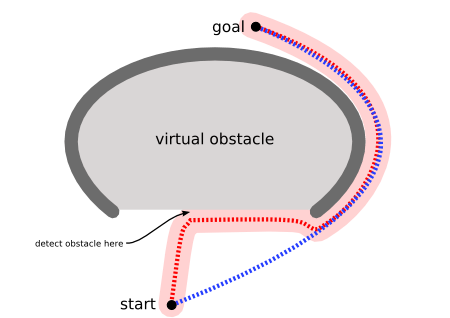
\includegraphics[width=0.48\textwidth]{concave2.png}
 	\caption{Algoritmo pathfinding.}
 	\label{concave2}
 \end{figure}

 \begin{figure}[H]
 	\centering
 	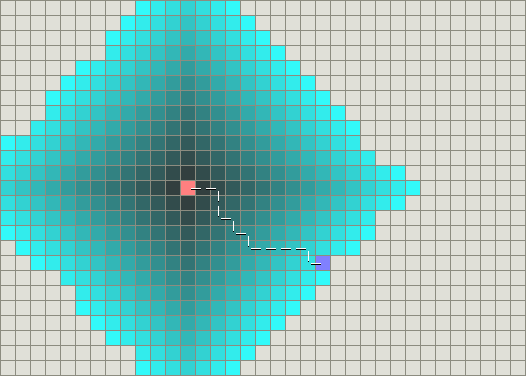
\includegraphics[width=0.48\textwidth]{dijkstra.png}
 	\caption{Algoritmo pathfinding.}
 	\label{dijkstra}
 \end{figure}
 
  \begin{figure}[H]
 	\centering
 	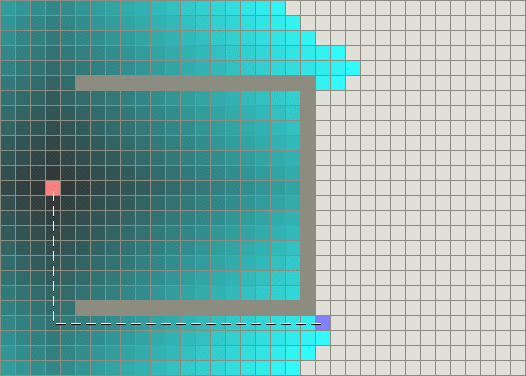
\includegraphics[width=0.48\textwidth]{dijkstra-trap.png}
 	\caption{Algoritmo pathfinding.}
 	\label{dijkstra-trap}
 \end{figure}
 
  \begin{figure}[H]
 	\centering
 	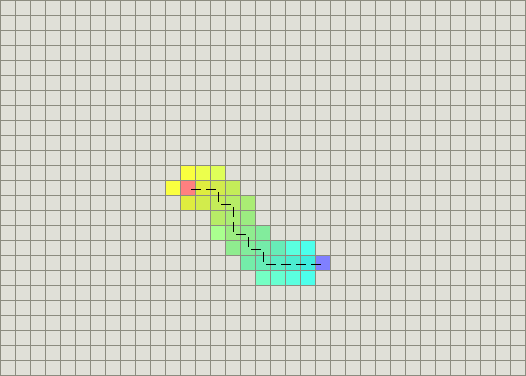
\includegraphics[width=0.48\textwidth]{a-star.png}
 	\caption{Algoritmo pathfinding.}
 	\label{a}
 \end{figure}
 
   \begin{figure}[H]
 	\centering
 	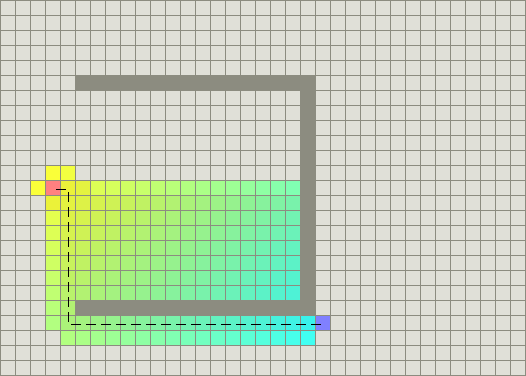
\includegraphics[width=0.48\textwidth]{a-star-trap.png}
 	\caption{Algoritmo pathfinding.}
 	\label{a-trap}
 \end{figure}

\section{Implementación}

\section{Trabajo a futuro}

\section{Conclusiones}




\section{Conclusiones}
A pesar de las diferentes arquitecturas de memorias basadas en RRAM reportadas en la literatura, no ha sido reportada una celda que logre una implementación funcional debido los problemas derivados de la variabilidad de los dispositivos.
  
\bibliographystyle{unsrtnat}
\nocite{*}
\bibliography{citas}% Produces the bibliography via BibTeX.

\end{document}
